\documentclass[aspectratio=169,12pt]{beamer}
\usetheme{Madrid}
\usecolortheme{default}

\usepackage{amsmath,amssymb,amsthm}
\usepackage{graphicx}
\usepackage{tikz}
\usetikzlibrary{arrows,positioning,shapes}

\title{Lightning Network Economics: Channels}
\subtitle{When Should Two Parties Use a Payment Channel?}
\author{Guasoni, Huberman, and Shikhelman (2024)}
\date{Presented By : Sravanth Potluri und5uv}

\begin{document}

\frame{\titlepage}

% ============================================
% SLIDE 1: Motivation
% ============================================
\begin{frame}{The Bitcoin Scalability Problem}
\begin{columns}
\begin{column}{0.5\textwidth}
\textbf{Bitcoin's Limitations:}
\begin{itemize}
    \item $\sim$7 transactions/second
    \item High fees during congestion
    \item Slow confirmation times
\end{itemize}

\vspace{0.5cm}
\textbf{Compare to:}
\begin{itemize}
    \item Visa: $\sim$65,000 tps
    \item Credit cards: instant settlement
\end{itemize}
\end{column}

\begin{column}{0.5\textwidth}
% PLACEHOLDER: Insert image of Bitcoin blockchain congestion graph
\end{column}
\end{columns}

\vspace{0.3cm}
\textbf{Key Question:} How can we scale Bitcoin without changing the base protocol?
\end{frame}

% ============================================
% SLIDE 2: The Lightning Network Solution
% ============================================
\begin{frame}{Enter the Lightning Network}
\textbf{Core Idea:} Move transactions \textit{off-chain}

\begin{center}
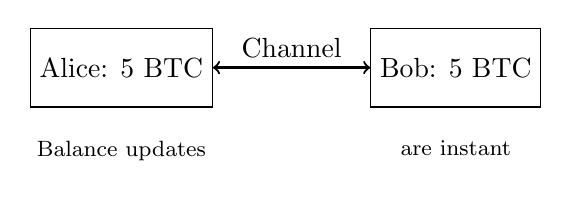
\begin{tikzpicture}[node distance=2cm, auto]
    \node[rectangle, draw, minimum width=2cm, minimum height=1cm] (alice) {Alice: 5 BTC};
    \node[rectangle, draw, minimum width=2cm, minimum height=1cm, right=of alice] (bob) {Bob: 5 BTC};
    \draw[<->, thick] (alice) -- node[above] {Channel} (bob);
    \node[below=0.3cm of alice] {\footnotesize Balance updates};
    \node[below=0.3cm of bob] {\footnotesize are instant};
\end{tikzpicture}
\end{center}

\textbf{How it works:}
\begin{enumerate}
    \item Open channel: one on-chain transaction
    \item Exchange unlimited payments off-chain
    \item Close channel: one on-chain transaction
\end{enumerate}

\textbf{Trade-off:} Save on transaction fees $\leftrightarrow$ Lock up capital
\end{frame}

% ============================================
% SLIDE 3: Real-World Analogy
% ============================================
\begin{frame}{Analogy: The Office Coffee Pool}
\begin{columns}
\begin{column}{0.5\textwidth}
\textbf{Inefficient Approach:}
\begin{itemize}
    \item Pay \$3 each morning
    \item \$1 transaction fee each time
    \item 20 workdays = \$20 in fees
\end{itemize}

\vspace{0.3cm}
\textbf{Efficient Approach:}
\begin{itemize}
    \item Prepay \$60 monthly
    \item \$1 fee twice (in \& out)
    \item Save \$18 in fees
    \item But: lock up \$60 for a month
\end{itemize}
\end{column}

\begin{column}{0.5\textwidth}

\vspace{0.5cm}
\textbf{Lightning channels face the same trade-off}
\end{column}
\end{columns}
\end{frame}

% ============================================
% SLIDE 4: The Model Setup
% ============================================
\begin{frame}{Formalizing the Problem}
\textbf{Two nodes} exchange payments over time

\textbf{Parameters:}
\begin{itemize}
    \item $\lambda_1$: Alice pays Bob at rate $\lambda_1$ (payments/time)
    \item $\lambda_2$: Bob pays Alice at rate $\lambda_2$ (payments/time)
    \item $C$: cost of one on-chain transaction
    \item $B$: cost to open/close a channel (round-trip)
    \item $r$: interest rate (opportunity cost of locked capital)
    \item $l_1, l_2$: collateral committed by each party
\end{itemize}

\vspace{0.3cm}
\textbf{Key Assumption:} Payments arrive as Poisson processes (random timing)

\vspace{0.3cm}
\textbf{Central Question:} When is a channel cheaper than on-chain payments?
\end{frame}

% ============================================
% SLIDE 5: Three Payment Strategies
% ============================================
\begin{frame}{Three Ways to Pay}
\begin{enumerate}
    \item \textbf{All On-Chain}
    \begin{itemize}
        \item No capital locked
        \item Cost: $C(\lambda_1 + \lambda_2)/r$
        \item Simple but expensive at high volume
    \end{itemize}
    
    \vspace{0.3cm}
    \item \textbf{Unidirectional Channel}
    \begin{itemize}
        \item Only one party makes payments through channel
        \item Other party pays on-chain
        \item Good when $\lambda_1 \gg \lambda_2$ (or vice versa)
    \end{itemize}
    
    \vspace{0.3cm}
    \item \textbf{Bidirectional Channel}
    \begin{itemize}
        \item Both parties make payments through channel
        \item Benefits from \textit{netting} opposing flows
        \item Best when $\lambda_1 \approx \lambda_2$
    \end{itemize}
\end{enumerate}
\end{frame}

% ============================================
% SLIDE 6: Intuition for Channel Costs
% ============================================
\begin{frame}{Understanding Channel Costs}
\textbf{A channel has two types of costs:}

\begin{enumerate}
    \item \textbf{Opening/Closing Cost:} $B$
    \begin{itemize}
        \item Fixed cost to set up channel
        \item Amortized over channel lifetime
        \item Want: longer channel lifetime $\Rightarrow$ larger collateral
    \end{itemize}
    
    \vspace{0.3cm}
    \item \textbf{Opportunity Cost:} $r \times (l_1 + l_2)$
    \begin{itemize}
        \item Capital locked in channel can't be used elsewhere
        \item Want: smaller collateral
    \end{itemize}
\end{enumerate}

\vspace{0.5cm}
\begin{center}
\textbf{Trade-off:} \\
Large collateral = long lifetime, low reset costs \\
Small collateral = high opportunity cost savings
\end{center}
\end{frame}

% ============================================
% SLIDE 7: Main Result 1 - Unidirectional
% ============================================
\begin{frame}{Main Result: Unidirectional Channels}
\textbf{Setting:} Alice pays Bob at rate $\lambda$, Bob never pays Alice

\begin{block}{Theorem (Asymptotic Cost for $r \to 0$)}
Optimal channel size: $l_2^* = \sqrt{B\lambda/r}$ \\[0.2cm]
Minimal cost: $c^* = 2\sqrt{B\lambda/r} - B/2 + O(r^{1/2})$
\end{block}

\textbf{Key Insights:}
\begin{itemize}
    \item Cost scales as $\boxed{r^{-1/2}}$ (square root scaling)
    \item Optimal collateral also scales as $r^{-1/2}$
    \item As interest rate $\downarrow$, should commit more capital
    \item As payment rate $\uparrow$, should commit more capital
\end{itemize}

\end{frame}

% ============================================
% SLIDE 8: Main Result 2 - Symmetric Bidirectional
% ============================================
\begin{frame}{Main Result: Symmetric Bidirectional Channels}
\textbf{Setting:} Both parties pay each other at rate $\lambda$

\begin{block}{Theorem (Asymptotic Cost for $r \to 0$)}
Optimal channel sizes: $l_1^* = l_2^* = (2B\lambda/r)^{1/3} + O(r^{1/3})$ \\[0.2cm]
Minimal cost: $c^* = 3(2B\lambda/r)^{1/3} - B/6 + O(r^{1/3})$
\end{block}

\textbf{Key Insights:}
\begin{itemize}
    \item Cost scales as $\boxed{r^{-1/3}}$ (cubic root scaling)
    \item \textbf{Much better than unidirectional!} ($-1/3$ vs $-1/2$)
    \item Benefit from \textit{netting}: opposing flows cancel out
    \item Both parties commit capital
\end{itemize}

\end{frame}

% ============================================
% SLIDE 9: Comparing Scalings
% ============================================
\begin{frame}{Why Does Bidirectional Scale Better?}
\begin{center}
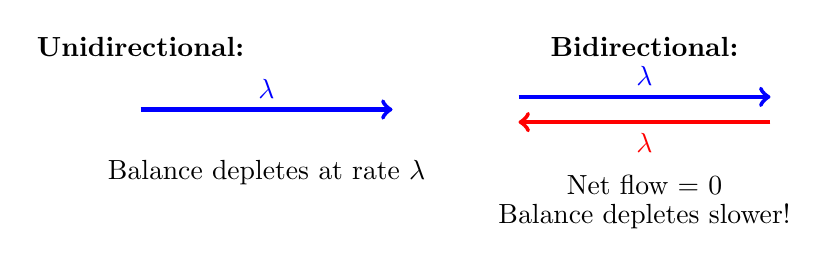
\begin{tikzpicture}[scale=0.8]
    % Unidirectional flow
    \node at (0, 3) {\textbf{Unidirectional:}};
    \draw[->, ultra thick, blue] (0, 2) -- (4, 2) node[midway, above] {$\lambda$};
    \node at (2, 1) {Balance depletes at rate $\lambda$};
    
    % Bidirectional flow
    \node at (8, 3) {\textbf{Bidirectional:}};
    \draw[->, ultra thick, blue] (6, 2.2) -- (10, 2.2) node[midway, above] {$\lambda$};
    \draw[->, ultra thick, red] (10, 1.8) -- (6, 1.8) node[midway, below] {$\lambda$};
    \node at (8, 0.8) {Net flow = 0};
    \node at (8, 0.3) {Balance depletes slower!};
\end{tikzpicture}
\end{center}

\textbf{Mathematical reason:}
\begin{itemize}
    \item Unidirectional: Balance follows one-sided random walk
    \item Bidirectional: Balance follows two-sided random walk
    \item Takes longer to hit boundary $\Rightarrow$ longer lifetime $\Rightarrow$ lower cost
\end{itemize}
\end{frame}

% ============================================
% SLIDE 10: Asymmetric Bidirectional
% ============================================
\begin{frame}{Asymmetric Bidirectional Channels}
\textbf{Setting:} $\lambda_2 > \lambda_1 > 0$ (unequal payment rates)

\begin{block}{Theorem (Asymptotic Cost for $r \to 0$)}
If $l_2 = O(r^{-1/2})$ and $l_1 = O(\log(r^{-1}))$, then: \\[0.2cm]
Minimal cost: $c^* = 2\sqrt{B(\lambda_2-\lambda_1)/r} + \frac{1 + \log(1 + \sqrt{B(\lambda_2-\lambda_1)/r} \cdot \log(\lambda_2/\lambda_1))}{\log(\lambda_2/\lambda_1)} + O(1)$
\end{block}

\textbf{Key Insights:}
\begin{itemize}
    \item Cost scales as $\boxed{r^{-1/2}}$ (like unidirectional!)
    \item Asymmetric channels behave like unidirectional with flow $\lambda_2 - \lambda_1$
    \item Average payer commits $O(r^{-1/2})$ capital
    \item Average payee commits only $O(\log(r^{-1}))$ capital
    \item Netting benefit exists but doesn't change scaling
\end{itemize}
\end{frame}

% ============================================
% SLIDE 11: The Big Picture
% ============================================
\begin{frame}{Synthesis: When to Use Which Channel?}
\begin{center}
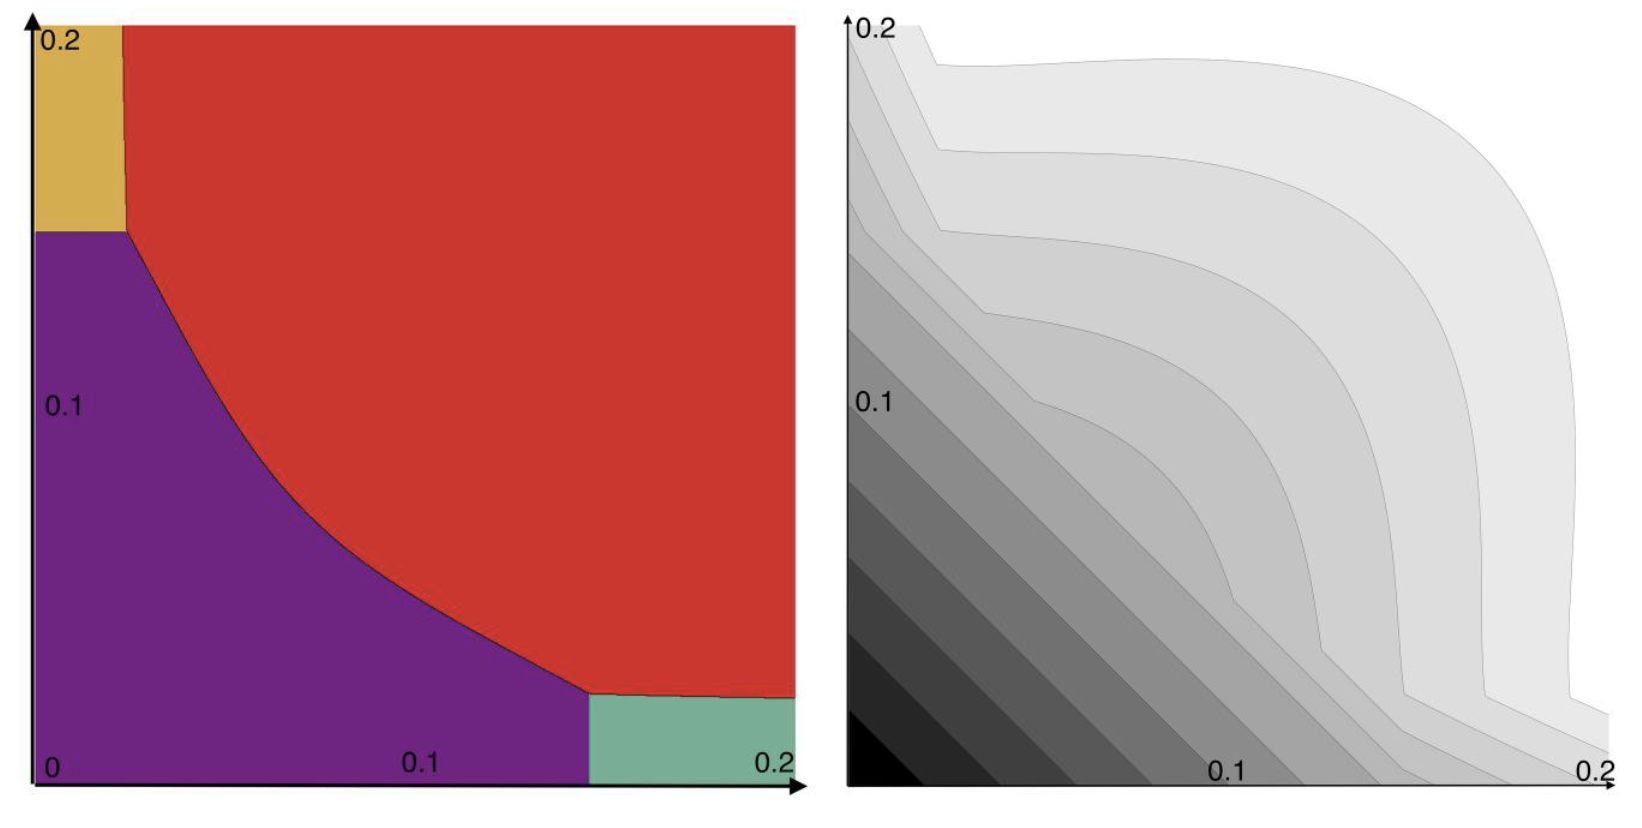
\includegraphics[width=0.5\textwidth]{Screenshot 2025-11-06 at 11.40.00 AM.png}
\end{center}

\textbf{Four regions in $(\lambda_1, \lambda_2)$ space:}
\begin{enumerate}
    \item \textbf{Bottom-left:} Both rates low $\Rightarrow$ All on-chain
    \item \textbf{Top-left/Bottom-right:} One rate high $\Rightarrow$ Unidirectional
    \item \textbf{Top-right:} Both rates high $\Rightarrow$ Bidirectional
    \item \textbf{Transition zones:} Hybrid strategies
\end{enumerate}
\end{frame}

% ============================================
% SLIDE 12: Necessary Conditions
% ============================================
\begin{frame}{When Are Channels Worth It?}
\textbf{Necessary conditions for channel optimality:}

\begin{block}{Theorem (Lower Bounds on Payment Rates)}
\begin{enumerate}
    \item Unidirectional channel: $C > \frac{Br}{\lambda} + o(r)$
    \item Bidirectional symmetric: $C > 3(\frac{Br^2}{4\lambda^2})^\frac{1}{3} - \frac{Br}{12\lambda} + o(r)$
\end{enumerate}
\end{block}

\textbf{Interpretation:}
\begin{itemize}
    \item Channels only worth it when:
    \begin{itemize}
        \item On-chain costs ($C$) are high, or
        \item Channel reset costs ($B$) are low, or
        \item Payment rates ($\lambda$) are high, or
        \item Interest rates ($r$) are low
    \end{itemize}
\end{itemize}
\end{frame}

% ============================================
% SLIDE 13: Congestion Reduction
% ============================================
\begin{frame}{Impact on Blockchain Congestion}
\textbf{Key Question:} How many on-chain transactions do channels save?

\begin{block}{Proposition (Congestion Reduction)}
Long-run ratio of channel transactions to on-chain transactions:
\begin{itemize}
    \item Unidirectional: $l_1$ (linear in collateral)
    \item Symmetric bidirectional: $l_1 l_2$ (product of collaterals!)
\end{itemize}
\end{block}

\textbf{Example:} $l_1 = l_2 = 10$
\begin{itemize}
    \item Unidirectional: 10 channel txs per on-chain tx
    \item Bidirectional: 100 channel txs per on-chain tx
\end{itemize}

\vspace{0.3cm}
\textbf{Implication:} Symmetric bidirectional channels provide \textit{quadratic} reduction in blockchain load!
\end{frame}

% ============================================
% SLIDE 14: Technical Innovation
% ============================================
\begin{frame}{Technical Contribution: The Model}
\textbf{This paper adapts classic inventory models to cryptocurrencies:}

\begin{columns}
\begin{column}{0.5\textwidth}
\textbf{Baumol-Tobin (1952-56):}
\begin{itemize}
    \item Demand for cash
    \item Transaction costs vs opportunity cost
    \item Inspired unidirectional analysis
\end{itemize}

\vspace{0.3cm}
\textbf{Miller-Orr (1966):}
\begin{itemize}
    \item Firm cash management
    \item Two-sided random walk
    \item Inspired bidirectional analysis
\end{itemize}
\end{column}

\begin{column}{0.5\textwidth}
\textbf{Key differences:}
\begin{itemize}
    \item Can always transact on-chain (alternative exists)
    \item Both cost and value storage
    \item Network effects matter
    \item Dynamic topology
\end{itemize}
\end{column}
\end{columns}

\vspace{0.3cm}
\textbf{Mathematical tool:} Difference equations with boundary conditions
\end{frame}

% % ============================================
% % SLIDE 15: Proof Sketch - Unidirectional
% % ============================================
% \begin{frame}{Proof Sketch: Unidirectional Channel Cost}
% \textbf{Key steps:}

% \begin{enumerate}
%     \item Model balance as Poisson process: payments arrive at rate $\lambda$
%     \item Expected cost satisfies difference equation:
%     \[J(n) = (l_1 + l_2)\frac{r}{r+\lambda_2+\lambda_1} + J(n+1)\frac{\lambda_2}{r+\lambda_2+\lambda_1} + \ldots\]
%     \item Boundary condition: $J(l_2) = J(0) + B$ (reset when depleted)
%     \item Solve to get exact formula (Theorem 1)
%     \item Take $r \to 0$ limit: $J(0) \approx \frac{B\lambda}{rl_2} + l_2 - \frac{B(l_2-1)}{2l_2}$
%     \item Optimize over $l_2$: $\frac{\partial J}{\partial l_2} = 0$
%     \item Yields $l_2^* = \sqrt{B\lambda/r}$ and cost formula
% \end{enumerate}
% \end{frame}

% % ============================================
% % SLIDE 16: Proof Sketch - Bidirectional
% % ============================================
% \begin{frame}{Proof Sketch: Bidirectional Channel Cost}
% \textbf{More complex due to two-sided random walk:}

% \begin{enumerate}
%     \item Balance evolves as $X_t = N_t^{\lambda_2} - N_t^{\lambda_1}$ (difference of Poisson)
%     \item Two boundaries: $-l_1$ (Alice exhausted) and $+l_2$ (Bob exhausted)
%     \item General solution involves eigenvalues:
%     \[\alpha_\pm = \frac{\lambda_1 + \lambda_2 + r \pm \sqrt{(\lambda_2-\lambda_1)^2 + r^2 + 2r(\lambda_2+\lambda_1)}}{2\lambda_2}\]
%     \item Cost function: $J(n) = l_1 + l_2 - B\frac{(\alpha_-^{l_1+l_2}-1)\alpha_+^{n} + (\alpha_+^{l_1+l_2}-1)\alpha_-^{n}}{\ldots}$
%     \item Asymptotic analysis as $r \to 0$:
%     \begin{itemize}
%         \item Symmetric: both eigenvalues approach 1, delicate cancellation
%         \item Asymmetric: one eigenvalue dominates
%     \end{itemize}
% \end{enumerate}
% \end{frame}

% ============================================
% SLIDE 17: Novel Insights
% ============================================
\begin{frame}{What's Really New Here?}
\textbf{Beyond adapting classic models:}

\begin{enumerate}
    \item \textbf{Scaling laws:} $r^{-1/2}$ vs $r^{-1/3}$ characterize fundamental difference
    \begin{itemize}
        \item Not obvious from Baumol-Tobin or Miller-Orr
        \item Shows power of symmetry/netting
    \end{itemize}
    
    \vspace{0.2cm}
    \item \textbf{Asymmetric analysis:} Logarithmic collateral for payee
    \begin{itemize}
        \item Surprising result: payee commits almost nothing
        \item Shows channels can be very asymmetric
    \end{itemize}
    
    \vspace{0.2cm}
    \item \textbf{Necessary conditions:}
    \begin{itemize}
        \item Quantifies when channels are viable
        \item Guides network design
    \end{itemize}
    
    \vspace{0.2cm}
    \item \textbf{Congestion reduction:} Quadratic for symmetric bidirectional
    \begin{itemize}
        \item Shows dramatic scalability improvement
        \item Justifies Lightning Network development
    \end{itemize}
\end{enumerate}
\end{frame}

% ============================================
% SLIDE 18: Limitations and Extensions
% ============================================
\begin{frame}{What's Missing?}
\textbf{Model limitations:}
\begin{itemize}
    \item Unit transaction size (simplified)
    \item Fixed costs $B, C$ (actually depend on congestion)
    \item Two-party channels (network effects not modeled)
    \item Poisson arrivals (may not capture all patterns)
    \item No routing fees
    \item No strategic behavior
\end{itemize}

\vspace{0.5cm}
\textbf{Companion paper} (Guasoni, Huberman, Shikhelman 2023):
\begin{itemize}
    \item Analyzes Lightning Network \textit{topology}
    \item How should channels connect?
    \item Optimal network structures
\end{itemize}
\end{frame}

% ============================================
% SLIDE 19: Empirical Questions
% ============================================
\begin{frame}{Testing the Theory}
\textbf{What would we observe if this model is right?}

\begin{enumerate}
    \item Channel sizes should scale as $r^{-1/2}$ (unidirectional) or $r^{-1/3}$ (bidirectional)
    \item Symmetric channels should be larger and last longer
    \item Channels should be rare when payment rates are low
    \item Average payees should commit less than average payers
\end{enumerate}

\vspace{0.5cm}
\textbf{Challenges for empirical testing:}
\begin{itemize}
    \item Can't observe payment rates directly (privacy!)
    \item Channel sizes are public but balances are not
    \item Interest rate $r$ unclear (opportunity cost subjective)
    \item Selection effects: who uses Lightning?
\end{itemize}
\end{frame}

% ============================================
% SLIDE 20: Discussion Questions
% ============================================
\begin{frame}{Discussion Questions}
\begin{enumerate}
    \item The model assumes payment rates are \textit{exogenous}. But wouldn't the existence of cheap channels \textit{increase} payment rates? How would endogenizing $\lambda$ change the results?
    
    \vspace{0.3cm}
    \item The paper treats $B$ and $C$ as fixed. But both depend on blockchain congestion, which channels reduce. Can the feedback loop be modeled? 
    
    \vspace{0.3cm}
    \item In the asymmetric case, the payee commits only $O(\log r^{-1})$ capital. Is this realistic? What might prevent such asymmetric arrangements?
    
    \vspace{0.3cm}
    \item The paper shows bidirectional channels reduce congestion quadratically. But if everyone uses bidirectional channels, what happens to the \textit{topology} of the network?
\end{enumerate}
\end{frame}

% ============================================
% SLIDE 21: Broader Implications
% ============================================
\begin{frame}{Beyond Bitcoin}
\textbf{This analysis applies to any layer-2 solution:}

\begin{itemize}
    \item Ethereum: Raiden Network, state channels
    \item Other cryptocurrencies: Liquid Network (Bitcoin), Polygon (Ethereum)
    \item Even traditional finance: settlement batching, clearinghouses
\end{itemize}

\vspace{0.5cm}
\textbf{General principle:} \\
When you have:
\begin{itemize}
    \item High per-transaction costs
    \item Frequent bilateral transactions
    \item Ability to cryptographically secure off-chain state
\end{itemize}
Then you should consider a channel-like solution

\vspace{0.5cm}
\textbf{This paper quantifies exactly when and how much you save}
\end{frame}

% ============================================
% SLIDE 22: Summary
% ============================================
\begin{frame}{Summary}
\textbf{Key takeaways:}
\begin{enumerate}
    \item Lightning channels trade off transaction costs for opportunity costs
    \item Unidirectional channels: cost $\sim r^{-1/2}$, good for one-way flows
    \item Bidirectional channels: cost $\sim r^{-1/3}$, much better for symmetric flows
    \item Asymmetric channels behave like unidirectional
    \item Channels viable when payment rates high, costs high, or interest rates low
    \item Symmetric bidirectional channels provide quadratic congestion reduction
\end{enumerate}

\vspace{0.5cm}
\textbf{Broader contribution:}
\begin{itemize}
    \item Rigorous economic foundation for Lightning Network
    \item Adapts classic inventory models to crypto context
    \item Provides design principles for layer-2 solutions
\end{itemize}
\end{frame}

\end{document}